\section{Mogan STEM: A WYSIWYG Structured Editor}
\label{sec:mogan}

Since last year, the maintainers of the Chinese TeXmacs community have developed Mogan STEM~\cite{moganstem2025} and a commercial version, Liii STEM~\cite{liiistem2025}, based on GNU TeXmacs. Currently, Mogan STEM and TeXmacs stand as the world's only WYSIWYG structured editors. Table~\ref{tab:mogan-vs-other} compares Mogan STEM with several other editors currently available on the market.

\begin{table}[htbp]
\centering
\caption{Comparison between Mogan STEM and alternative editors}
\label{tab:mogan-vs-other}
\begin{tabular}{lcccc}
\toprule
\textbf{Editor} & \textbf{WYSIWYG} & \textbf{Structured} & \textbf{Unicode Support} & \textbf{\TeX{} Compatibility} \\
\midrule
\textbf{Mogan STEM} & Yes & Yes & Yes & Partial \\
\textbf{TeXmacs} & Yes & Yes & Partial & Partial \\
\textbf{TeX/LaTeX} & No & Yes & Partial & Full \\
\textbf{Word} & Yes & No & Partial & Incompatible \\
\textbf{LyX} & Partial & Yes & Partial & Full \\
\textbf{Typst} & No & Yes & Yes & Partial \\
\bottomrule
\end{tabular}
\end{table}

The core technical challenge in achieving the WYSIWYG capability of Mogan STEM lies in the representation and rendering of mathematical formulas. Unlike \TeX{}, which represents formulas through layout-oriented markup in the form of typesetting instructions, Mogan STEM adopts a tree-based, functional representation for both mathematical formulas and the document structure itself. The following discussion evaluates this mechanism with specific examples.

\subsection{Tree-Structured Formulas and Document Structure}
\label{sec:tree-struc-on-mogan}

Unlike \LaTeX{}'s compilation model, which centers on linear text and macro expansion, TeXmacs features an explicit tree-based document structure designed from the outset. Document components---such as chapters, formulas, citations, and typesetting elements---exist as structured nodes, rather than being implicitly embedded within macro calls or token streams. This architectural distinction directly impacts citation updates, compilation efficiency, and the interactive user experience.

A fraction serves as a primary example of this difference. In \TeX{}, a fraction is represented as \verb|\frac{1}{2}|; internally, the compiler processes \verb|\frac|, \verb|{1}|, and \verb|{2}| serially. In Mogan STEM, however, the fraction is represented at the underlying layer as the Scheme code \verb|(frac "1" "2")|.\footnote{Note that Mogan STEM is \textbf{WYSIWYG}; therefore, when inputting $\frac{1}{2}$, the user does not type \texttt{(frac 1 2)}, but instead presses \keys{Alt + F} to input it visually!} This forms a tree structure, as illustrated in Figure~\ref{fig:frac-tree}.

\begin{figure}[htbp]
\centering
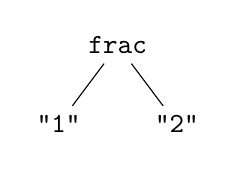
\begin{tikzpicture}[
    level 1/.style={sibling distance=15mm, level distance=10mm},
    every node/.style={align=center}
]
\node {\texttt{frac}}
    child {node {\texttt{"1"}}}
    child {node {\texttt{"2"}}};
\end{tikzpicture}
\caption{The Tree Structure of Mogan Formulas}
\label{fig:frac-tree}
\end{figure}

Let us consider another example:

\begin{equation}
\label{eq:tree-struc}
\int_{a}^{b} f(x) \mathrm{d}x = \left[ F(x) \right] \big|_{a}^{b}
\end{equation}

Its Scheme representation is as follows:
\begin{lstlisting}[caption={Scheme representation of integral expression},label={lst:scheme-integral},upquote=true]
> `(math (concat (big "int") (rsub "a") (rsup "b") "f" (around* "(" "x" ")") "<mathd>x=" (around* "<nobracket>" (around* "[" (concat "F" (around* "(" "x" ")")) "]") "|") (rsub "a") (rsup "b")))
\end{lstlisting}

Note that the segment $\left[ F(x) \right] |$ is managed via the tree structure illustrated in Figure~\ref{fig:tree-representation}. Consequently, even if a user omits a parenthesis or two, this omission does not negatively affect the rendering of the entire mathematical expression in Mogan.

\begin{figure}[htbp]
    \centering
    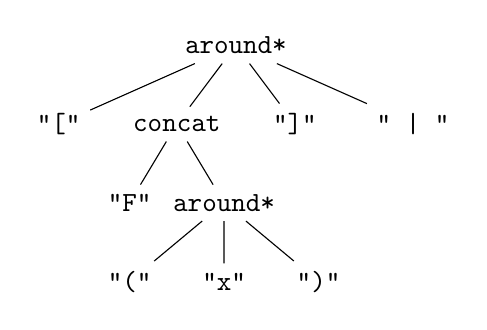
\begin{tikzpicture}[
        level 1/.style={sibling distance=15mm, level distance=10mm},
        level 2/.style={sibling distance=12mm, level distance=10mm},
        level 3/.style={sibling distance=12mm, level distance=10mm},
        every node/.style={align=center}
    ]
    \node {\texttt{around*}}
        child {node {\texttt{"["}}}
        child {node {\texttt{concat}}
            child {node {\texttt{"F"}}}
            child {node {\texttt{around*}}
                child {node {\texttt{"("}}}
                child {node {\texttt{"x"}}}
                child {node {\texttt{")"}}}
            }
        }
        child {node {\texttt{"]"}}}
        child {node {\texttt{" | "}}};
    \end{tikzpicture}
    \caption{Tree representation of $ [F (x)] |$}
    \label{fig:tree-representation}
\end{figure}

Unlike \TeX{}, this tree structure exists at the rendering level, not the syntax level. In fact, many long-time users of Mogan and TeXmacs cannot write a single line of Scheme code! This rendering-level tree structure offers two distinct advantages:

\begin{enumerate}
    \item \textbf{Local Scoping of Input Errors:}
    \begin{itemize}
        \item Errors do not cause the entire document to fail rendering (a major drawback of \LaTeX{}).
        \item Local edits do not trigger global layout instability (a major drawback of MS Word).
    \end{itemize}

    \item \textbf{Parallel Processing:} The CPU renders data in parallel rather than serially, which significantly accelerates rendering speed.
\end{enumerate}

Let's look at another example. For a two-line layout like Figure~\ref{fig:double-line}, the representation is:
\begin{lstlisting}
(document "Mogan Logo" "(figure )" (itemize (document (concat (item) "WYSIWYG Writing") "")))
\end{lstlisting}

\begin{figure}[htbp]
\centering
\includegraphics[width=0.3\textwidth]{figure/double-line.png}
\caption{Image insertion between lines}
\label{fig:double-line}
\end{figure}

\begin{figure}[htbp]
\centering
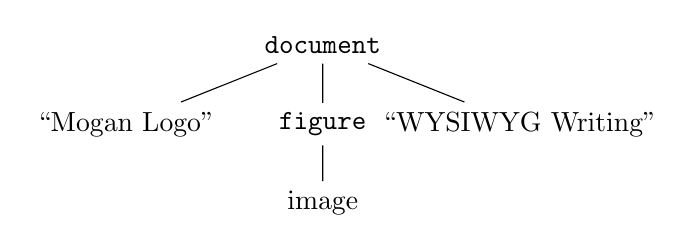
\begin{tikzpicture}[
    level 1/.style={sibling distance=25mm, level distance=10mm},
    level 2/.style={sibling distance=25mm, level distance=10mm},
    every node/.style={align=center}
]
\node {\texttt{document}}
    child {node {``Mogan Logo''}}
    child {node {\texttt{figure}}
        child {node {image}}
    }
    child {node {``WYSIWYG Writing''}};
\end{tikzpicture}
\caption{Mogan's multi-line data structure}
\label{fig:multiline-mogan}
\end{figure}

This corresponds to the tree structure shown in Figure~\ref{fig:multiline-mogan}. As the figure demonstrates, in Mogan, each line of content and every image block maps to an independent leaf node within the tree. Consequently, modifying an image (e.g., resizing or replacing it) triggers a re-render of only that specific leaf node, without disrupting the layout of surrounding lines. This design effectively resolves the issue common in unstructured editors such as Word, where local modifications often lead to global layout chaos.

\subsection{Functional Symbol Representation}

In \TeX{}, all mathematical symbols and fonts are represented as strings. However, in Mogan STEM, certain special symbols are defined via functions. For instance, the inner product $\langle \cdot \rangle$, as shown in Equation~\ref{eq:braket}, is an anonymous function that automatically scales according to the symbols it contains. While this is similar to \verb|\langle \rangle| in \LaTeX{}, the difference lies in the fact that, as a complete function, the left and right brackets always renders a unified pair rather than isolated characters. To obtain a single bracket, the user manually deletes the undesired character from the rendered pair.

\begin{equation}
\label{eq:braket}
\left\langle \int \right\rangle \langle f \rangle
\end{equation}

This functional approach contrasts with \LaTeX{}'s macro-based approach, where \verb|\frac{a}{b}| relies on positional arguments and implicit grouping.

\subsection{Fast Reference Rendering}

Taking bibliographic citations as an instance: in the \LaTeX{} ecosystem, \verb|\cite| serves merely as a macro interface, with actual citation relationships established indirectly via intermediate files such as \verb|.aux| and \verb|.bbl|. Consequently, any modification to bibliography entries typically necessitates multiple global compilation cycles, exemplifying a classic batch processing model. In contrast, Mogan STEM treats citation relationships as structural links directly embedded in the document tree. To update a reference, the system performs only a local search and re-renders the specific leaf nodes involved, thereby avoiding a full re-parsing of the document.

Cross-references in Mogan STEM are maintained as bidirectional links in the document tree. When a label is updated, all references to it are automatically updated without requiring a full recompilation. This provides immediate visual feedback and eliminates the need for multi-pass compilation.

\subsection{On-demand plugin loading}

Mogan adopts a monolithic installation paradigm, diverging from the package repository distribution model exemplified by TeX Live. Its installation package delivers a complete and self-contained editing and typesetting system, encompassing core executables, a built-in Scheme runtime, a document model, and a rendering engine. Consequently, users avoid managing numerous independent packages or resolving granular macro dependencies. Although functional extensions exist as plugins, they do not load upon startup; instead, they load dynamically at runtime only when specific document structures trigger the corresponding requirements. This on-demand mechanism ensures that system complexity is dictated by document content rather than a pre-configured feature set.

It is noteworthy that Mogan requires an installation package of merely one hundred megabytes, occupying only several hundred megabytes of local storage upon extraction, yet it offers immediate, out-of-the-box support for the editing and export of complex mathematical documents. In stark contrast, even a minimalist \LaTeX{} installation typically demands a local environment exceeding 1 GB, while a full distribution reaches approximately 6 GB in 2025.

This disparity stems from a fundamental divergence in system design. \LaTeX{} front-loads "potential future capabilities" as an installation cost, maintaining compatibility through its macro language and package ecosystem. Conversely, Mogan defers complexity to runtime, confining it within the actual execution path. It achieves extensibility via a unified document tree model and a runtime plugin mechanism. Consequently, Mogan's complexity activates dynamically by specific documents at runtime, whereas \LaTeX{}'s complexity manifests primarily during the installation and configuration phases.

In summary, TeX Live installs an ever-accumulating repository of historical packages, whereas Mogan installs an evolvable document system. The complexity of the former is front-loaded to the installation phase, while the latter is triggered by the document at runtime.

Mogan STEM's architecture supports on-demand loading of features and document types. Unlike \LaTeX{}, where the entire distribution must be installed upfront, Mogan loads only the components needed for the current document. This significantly reduces installation size and startup time.
